
\chapter{Representing changes | Note start 2023-04-05}
    Predicate calulus is insufficient to describe changes in the real world,
    it is \textit{static}. As solutions to these kinds of problems, temporal logics were developed. A simple example is \textit{Situational calculus}, where o each formula we also add the state in which it applies.
\chapter{Problem with the lack of information}
Logic--based methods presented complete knowledge about the system. Unfortunately, in the real world we rarely have complete information, and also, agents in the real world often act without information about the spefici situations they encounter. Said agents may however posses partial information, such as:
\begin{itemize}
        \item "typical" facts
        \item "Possible" facts
        \item "probable" facts 
        \item exceptions to usualy valid facts

\end{itemize}
Another problem is the reliability of data. In the real world, all information caries with t some degree of uncertainty. This information however should sitll be used to make decisions in the absence of perfect information, as it could still allow us to make a mostly correct decision.
\nt{Clasical vs Probabilistic logic}
{
    Classical logic does not provide any mechanisms for representing uncertainty and insufficiency in data. Probabilistic logic however, treats all predicates as probabilities, allowing it to better model the real world, at the cost of higher complexity.
}

\chapter{Probabilistic Logic}
    \section{Probability}
        Since in the real world all information is uncertain and incomplete, we want to create a model which accounts for these facts. There were multiple models developed for this purpouse, only recently however did they start being used in areas of \textit{Artificial Intelligence}.
        \dfn{Prior Probability}
        {
            Prior probability designates probability of an event occuring, without any information about factors affecting it, or any other information about the event(such as that it did in fact occur).
        }
        \nt{Probability as a whole}
        {
            Looking at it right now, it looks like it's just highschool level probability, De'Morgan laws aply, etc.
        }
        \ex{Some Probability Axioms}
        {
            \begin{itemize}
                    \item $P(\neg A) = 1 - P(A)$
                    \item $P(A) = P(A \wedge B) + P(B-A)$
                    
            \end{itemize}
        }

        \dfn{Random Variables}
        {
            A random variable represents some chance event, which may assume some values from a set. If we can associate with each of those values a probability of it occurin, we have a probability distribution.
        }
        \dfn{Joint probability distribution}
        {
            Consider severall variables representig several chance events. We can then create a sort of table(or high dimensional tensor), eg.
            \begin{center}
            \begin{tabular}{|c|c|c|c|c|}

            \hline
                 &$X = x_1$&$X = x_2$ & $\cdots $ &$X = x_n$ \\
            \hline
               $ Y = y_1$ & & & & \\
            \hline
                $Y = y_2$ & & & & \\
            \hline
                $\cdots $ & & & & \\
            \hline
                $Y = y_n $ & & & & \\
            \hline
            \end{tabular}
            \end{center}    
            This is esentially a 2d function, with its values summing up to 1.
            
        }

        \dfn{Conditional Probability}
        {
            $P(A\mid B)$ -- Probability of A accuring, given that B occurs. In terms of prior probability:
            $P(A\mid B) = \frac{P(A \wedge B)}{P(B)}$
        }

        \ex{Some laws of conditional probability}
        {
            \begin{itemize}
                    \item $P(A) = P(A\mid B)P(B) + P(A \mid \neg B)P( \neg B)$
                    \item $P(A \mid B) + P(A \mid \neg B) = 1$
                    
            \end{itemize}
        }

        \ex{Montey Hall problem}
        {
            Too much to write, not enough will. Something something, goat, car $ \frac{2}{3} $.
        }

        \ex{SARS test}
        {
            When testing for a rare disease, the usefullness of the dest depends both on it's accuracy, and the percentage of people infected in the tested population. An examle, assume that the test gives positive and correct results in 95 out of 100 cases. Moreover, it gives negative and correct results in 90 to 100, eg.
            \begin{itemize}
                    \item $P(SARS) = 0.0001$
                    \item $P( T^{+} \mid SARS) = 0.95$
                    \item $P(T ^{-} \mid \neg SARS) = 0.95$
            \end{itemize}
            Now find $P(SARS \mid T^{+})$

            \begin{enumerate}
            \item $P(T^{+}) = P(T^{+} \mid SARS)P(SARS) + P(T^{+} \neg SARS)P(\neg SARS)$
            \item $P(T^{+}) = 0.95 \times 0.0001 + 0.10 * 0.09999$
            \item  $P(T^+) = 0.100085$
            \end{enumerate}
            and finaly, we can compute $P(SARS \mid T^+)$
             \begin{equation}
                P(SARTS \mid T^+) = \frac{0.95 \times 0.0001}{0.00085} \approx 0.00095
            \end{equation}

        }

        \dfn{Causal vs Diagnostic knowldege}
        {
            Causal knowledge refers to the causal relations between events, for example, the virus \textit{causes} the test to give a positive result.
            Diagnostic knowledge is something else, not enough time $\cdots $
        }


 \chapter{Belief(Baysian) networks}
 
    Baysian networks are directed graphs representing various conditional probabilities. In this description, an event is represented by a node, and probablity of it triggering another node given its state is associated with each node. A causal relation is describd by a directed edge.
%% give a metwork example
    \begin{center}
        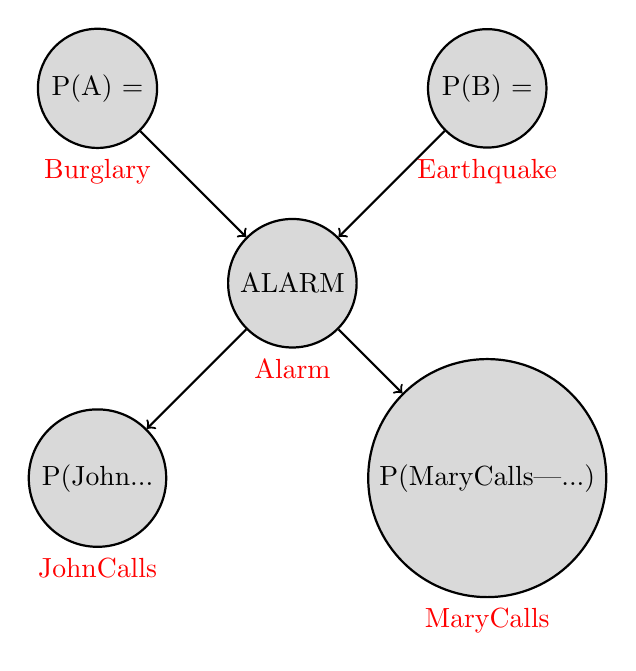
\begin{tikzpicture}[thick,node distance = {35mm},radius={15mm},  main/.style = {draw, circle}]
        \node[main, fill = gray!30, label={[red]below:Alarm}](1) {ALARM};
        \node[main, fill = gray!30, label={[red]below:Burglary}](2)[above left of=1] {P(A) = };
        \node[main, fill = gray!30, label={[red]below:Earthquake}](3)[above right of=1] {P(B) = };
        \node[main, fill = gray!30, label={[red]below:JohnCalls}](4)[below left of=1] {P(John...};
        \node[main, fill = gray!30, label={[red]below:MaryCalls}](5)[below right of=1] {P(MaryCalls|...)};
        
        \draw[->] (2) to [out=315, in=135, looseness=2.5] (1);
        \draw[->] (3) to [out=225, in=45, looseness=2.5] (1);
        \draw[->] (1) to [out=225, in=45, looseness=2.5] (4);
        \draw[->] (1) to [out=315, in=135, looseness=2.5] (5);
        
        
    \end{tikzpicture}
\end{center}
\section{Preferences and utility functions}

\dfn{Utility function}
{
    A utility function $U(S)$ designates states which are preferred by the agent. Such a designation is very subjective, and depends heavily on the agent.}
    \dfn{Expected utiliyu $EU(A)$}
    {
        Expected utility of a non deterministic action A with a set of possible results and associated probabilities is given as:
        \begin{equation}
            EU(A \mid E) = \Sigma_i P(Result_i(A)\mid Do(A),E) \times U(Result_i(A))
        \end{equation}
        where:
        \begin{itemize}
                \item A  -- non deterministic function
                \item $\{Result\}$
                
        \end{itemize}
    }


\section{Lotteries and preferences}
When the agent makes a decision under uncertain circumstances, we call this decision a lottery. The results of a latter is either a state, or another lottery.
\subsection{Utility Functions}
\nt{For a set of agent's preferences satisfying the preference axioms there exists a real valued function $U$ defined for the set of states $U\,:\,S \longrightarrow \mathbb{R} $.}

Something something expected utility principle...

\section{Making decisions}
    The Bayesian belief networks provide answers abot the probability distributions of any random variables, assuming proit knowledge about any combination of other variables. Given a utility distribution, we can infer this knowledge on the basis of MEH principle.
    \ex{2}{When leaving home, should w take an umbrella? It would be only useful in rain, otherwise it is annoying to carry. How do we know I its going to rain? We can check the weather forecast. What we have to understand, is that the forecast is unreliable, so we can only make a decision based on a preference(??)}

 \dfn{Influence diagrams}
 {
     Both the action to consider, and the utilities of the situation can be added to the belief network graph as spatial action and utility nodes. There should be links from appropriate chance nodes and action nodes to the utility nodes.
     Such extended belief networks are called \textit{Influence Diagrams} or else were  \textit{Decision networks}.
     \ex{1}
     {
         Consider that we have no additional information.
         GRAPH GRAPH GRAPH GRAPH!!!! 
         \begin{equation}
             EU(\text{leave}) = P(\text{sunny})*U(\text{leave,sunny})+P(\text{rainy})*U(\text{leave,rainy}) = \\
             0.7*100+\cdots 

         \end{equation}
         \begin{equation}
             EU(\text{take}) = P(\text{sunny})*U(\text{take,sunny})+P(\text{rainy})*U(\text{take,rainy}) = \\
             0.7*100+\cdots 

             
         \end{equation}
         So ultimately we choose to leave the umbrella, as it has lower utility.

         Suppose now that we do have some information, namely a bad weather forecast. Querying the network we get $P(\text{sunny,rainy}\mid \text{bad}) \approx (0.34,0.66)$. Then we have: %% NEW EQUATIONS WITH 

         \begin{equation}
             EU(\text{leave}) = P(\text{sunny})*U(\text{leave,sunny})+P(\text{rainy})*U(\text{leave,rainy}) = 0.34*100+0.66*0=0
         \end{equation}
         \begin{equation}
             EU(\text{take}) = P(\text{sunny})*U(\text{take,sunny})+P(\text{rainy})*U(\text{take,rainy}) = 0.34*20+0.66*70=53
         \end{equation}
         meaning that we do take the umbrella.
     }
 
 }




